\documentclass[12pt,a4paper,twoside]{article}

%\usepackage[utf8]{inputenc}
\usepackage[T1]{fontenc}
\usepackage[english]{babel}
\usepackage{lmodern}
\usepackage{tikz}
\usepackage{fontspec}
%\setmonofont{Inconsolata}
\setmonofont[Scale=0.85]{Source Code Pro}

\usetikzlibrary{shapes.geometric,positioning,calc,arrows}

\usepackage{listings}

\usepackage{amsmath, mathpartir, adjustbox}
\usepackage[labelformat=simple]{subfig}
\usepackage[font={sf},margin=10pt,labelfont=bf]{caption}
\usepackage{booktabs}
\usepackage[colorlinks=false]{hyperref}
\providecommand*{\listingautorefname}{Listing}

\usepackage{newunicodechar}
\newfontfamily{\freeserif}[Scale=MatchLowercase]{DejaVu Sans}
\newunicodechar{ℕ}{\freeserif{ℕ}}
\newunicodechar{ₐ}{\freeserif{ₐ}}
\newunicodechar{₁}{\freeserif{₁}}
\newunicodechar{∈}{\freeserif{∈}}
\newunicodechar{𝓞}{\ensuremath{\mathcal{O}}}
\newunicodechar{∉}{\freeserif{∉}}
%\newunicodechar{Π}{\freeserif{Π}}
%\newunicodechar{→}{\freeserif{→}}
\newunicodechar{⦃}{\freeserif{⦃}}
\newunicodechar{⦄}{\freeserif{⦄}}
\newunicodechar{∧}{\freeserif{∧}}
\newunicodechar{∨}{\freeserif{∨}}
\newunicodechar{⊢}{\freeserif{⊢}}
\newunicodechar{⊑}{\freeserif{⊑}}
\newunicodechar{ₚ}{\freeserif{ₚ}}
\newunicodechar{∘}{\freeserif{∘}}
\newunicodechar{ₗ}{\freeserif{ₗ}}

\usepackage{fancyhdr}
\setlength{\headheight}{15pt}
\usepackage{todonotes, rotating}
\usepackage{minted}
%workaround to remove red boxes
\renewcommand{\fcolorbox}[4][]{#4}
\usemintedstyle{tango}
\usemintedstyle[final]{bw}
\newmintinline[rust]{rust}{}
\newmintinline[lean]{lean}{}
\setminted{breaklines=true, fontsize=\footnotesize\linespread{0.85}}
\setmintedinline{fontsize=\normalsize}

\clubpenalty = 10000
\widowpenalty = 10000 \displaywidowpenalty = 10000

\begin{document}

\def\sectionautorefname{Section}
\def\subsectionautorefname{Subsection}
\def\subsubsectionautorefname{Subsection}

\newenvironment{sbs1}{%
  \vspace{1em}\noindent\minipage[t]{0.36\textwidth}%
  \minted{rust}}{%
  \endminted\endminipage}
\newenvironment{sbs2}{%
  \hfill\vline\hfill%
  \minipage[t]{0.62\textwidth}%
  \minted{lean}}{%
  \endminted\endminipage\vspace{1em}}

\newcommand\ie{i.e.\ }
\newcommand\eg{e.g.\ }

  \begin{titlepage}
    \begin{tikzpicture}[remember picture,overlay]
      % Seitenrahmen zeichnen.
      \draw[semithick,rounded corners=0.5cm]
        ($(current page.north west) + ( 1cm,-1cm)$) --
        ($(current page.north east) + (-1cm,-1cm)$) --
        ($(current page.south east) + (-1cm, 1.5cm)$);

      \draw[semithick,rounded corners=0.5cm]
        ($(current page.south east) + (-1cm, 1.5cm)$) --
        ($(current page.south west) + ( 1cm, 1.5cm)$) --
        ($(current page.north west) + ( 1cm,-1cm)$);

      % Logo einbinden.
      \node[anchor=north west] (logo) at ($(current page.north west) + (1.75cm,-1.5cm)$)
      {
        
\includegraphics[width=4cm]{KITLogo}
      };

      % Institut / Lehrstuhl.
      \node[anchor=east] at ($(current page.east |- logo.east) + (-1.75cm,0cm)$)
      {
        \begin{minipage}[t]{5.2cm}
          \begin{flushleft}
            \footnotesize{}Institut für Programmstrukturen und Datenorganisation (IPD) \\
            \vspace{6pt}
            Lehrstuhl Prof.\ Dr.-Ing.\ Snelting
          \end{flushleft}
        \end{minipage}
      };

      \node (title) at ($(current page.center |- logo.south) + (0cm, -4cm)$)
      {
        % Korrekter Zeilenabstand etc. durch Minipage.
        \begin{minipage}[t]{12cm}
          \begin{center}
            \huge\textbf{Simple Verification of Rust Programs via Functional Purification}
          \end{center}
        \end{minipage}
      };

      \node[below=1.75cm of title.south]   (prename)  { Masterarbeit von };
      \node[below=0.75cm of prename.south] (name)     { \Large{}\textbf{Sebastian Ullrich} };
      \node[below=1cm    of name.south]    (postname) { an der Fakultät für Informatik };

      \node[below=3cm    of name.south]    (bildchen) { 
\includegraphics[width=0.9\textwidth]{logo.png}
                                                      };

      \node[below=2cm of bildchen.south] (table)
      {
        \begin{tabular}{ll}
          \textbf{Erstgutachter:}           & Prof.\ Dr.-Ing.\ Gregor Snelting \\[5pt]
          \textbf{Zweitgutachter:}          & ??? \\[5pt]
        \end{tabular}
      };

      \node[below=3.5cm of table.south] (time)
      {
        \begin{tabular}{ll}
        \textbf{Bearbeitungszeit:} & 4. Juli 2013 -- 29. Oktober 2013
        \end{tabular}
      };

      % Fußzeile, unten zentriert.
      \node[anchor=south] (footnote) at ($(current page.center |- current page.south) + (0cm, 0.65cm)$)
      {
        \tiny{}KIT -- Universität des Landes Baden-Württemberg und nationales Forschungszentrum in der Helmholtz-Gemeinschaft
        \hspace{0.5cm}
        \Large{}\textbf{www.kit.edu}
      };
    \end{tikzpicture}
  \end{titlepage}

% sane default for proof documents
%\parindent 0pt\parskip 0.5ex

\tikzset{every node/.style={transform shape},auto,block/.style={align=center,rectangle,draw,minimum height=20pt,minimum width=30pt},>=triangle 60}
%\pagenumbering{Roman}
\pagestyle{empty}
\renewcommand{\abstractname}{Einfache Verifikation von Rust-Programmen}
\begin{abstract}
  Imperative Programmiersprachen sind in der modernen Softwareentwicklung
  allgegenwärtig, stellen aber ein Hindernis für formale Softwareverifikation
  dar durch ihre Verwendung von veränderbaren Variablen und Objekten. Programme
  in diesen Sprachen können normalerweise nicht direkt auf die unveränderliche
  Welt von Logik und Mathematik zurückgeführt werden, sondern müssen in eine
  explizit modellierte Semantik der jeweiligen Sprache eingebettet werden. Diese
  Indirektion stellt ein Problem für die Benutzung von interaktiven
  Theorembeweisern dar, da sie die Entwicklung von neuen Werkzeugen, Taktiken
  und Logiken für diese ``innere'' Sprache bedingt.

  Die vorliegende Arbeit stellt einen Compiler von der imperativen
  Programmiersprache Rust in die pur funktionale Sprache des Theorembeweisers
  Lean vor, der nicht nur generell das erste Werkzeug zur Verifikation von Rust-Programmen
  darstellt, sondern diese insbesondere auch
  mithilfe der von Lean bereitgestellten Standardwerkzeugen und -logik
  ermöglicht. Diese Transformation ist nur möglich durch spezielle Eigenschaften
  von allen validen Rust-Programmen, die die Veränderbarkeit von Werten auf
  begrenzte Geltungsbereiche einschränken und statisch durch Rusts Typsystem
  garantiert werden. Die Arbeit demonstriert den Einsatz des Compilers anhand
  der Verifikation von Realbeispielen und zeigt die Erweiterbarkeit des Projekts
  über reine Verifikation hinaus am Beispiel von asymptotischer Laufzeitanalyse auf.
\end{abstract}
\renewcommand{\abstractname}{Abstract}

\newpage

\begin{abstract}
Imperative programming, and aliasing in particular, represents a major
obstacle in formally reasoning about everyday code. By utilizing restrictions
the imperative programming language Rust imposes on mutable aliasing, we
present a scheme for shallowly embedding a substantial part of the Rust language into the
purely functional language of the Lean theorem prover. We use this scheme to
verify the correctness of real-world examples of Rust code without the need
for special semantics or logics. We furthermore
show the extensibility of our transformation by incorporating an analysis of
asymptotic runtimes.
\end{abstract}
\tableofcontents

\cleardoublepage
\pagestyle{fancy}
\fancyhf{}
\fancyhead[LE,RO]{\thepage}
\fancyhead[RE,LO]{\textit\leftmark}
\pagenumbering{arabic}

\section{Introduction}

Imperative programming languages are ubiquitous in today's software development,
making them prime targets for formal reasoning. Unfortunately, their semantics
differ from those of mathematics and logic -- the languages of formal methods -- in some
significant details, starting with the very concept of ``variables''. The problem
of mutability is only exacerbated for languages that allow references to
\emph{alias}, or point to the same memory location, enabling non-local mutation.

The standard way of verifying programs in such languages with the help of an
interactive theorem prover is to explicitly model the semantics of the language
in the language of the theorem prover, then translate
the program to this representation (a ``deep'' embedding) and finally prove the
correctness of its formalized behavior. This general approach is very flexible
and allows for the verification of meta programs such as program transformations.
The downside of the approach is that the theorem prover's tools and tactics may
not be directly applicable to the embedded language, defeating many amenities of
modern theorem provers.
Alternatively, programs can be ``shallowly'' embedded by directly translating them
into terms in the theorem prover's language without the use of an explicit inner semantics.
This simplifies many semantic details such as the identification and
substitution of bound variables, but it is harder to accomplish the more the semantics
of the source language differs from the theorem prover's own semantics.

Regardless of the type of embedding,
an explicit heap that references can point into must generally be modeled and
passed around in order to deal with the aliasing problem. References in this model may be as simple as
indices into a uniform heap, but various logics such as separation logic~\cite{reynolds2002separation} have been developed to work on a more abstract representation and to express
aliasing-free sets of references.

Languages with more restricted forms of aliasing exist, however.
Rust~\cite{matsakis2014rust}, a new, imperative systems programming language,
imposes on mutable references the restriction of never being aliased by any
other reference, mutable or immutable. This restriction eliminates the
possibility of data races and other common bugs created by the presence of
mutable sharing such as iterator invalidation. It furthermore enables more
aggressive optimizations.

While the full Rust language also provides raw pointers, which are not bound by
the aliasing restriction, and other ``unsafe'' operations, a
memory model for Rust (informal or formal) has yet to be proposed. We therefore focus on the ``safe''
subset of Rust that has no unsolved semantic details.

We utilize safe Rust's aliasing restriction to design a monadic shallow embedding of a
substantial subset of Rust
into the purely functional language of the Lean~\cite{de2015lean} theorem prover, without the need
for any heap-like indirection. This allows us to
reason about unannotated, real-world Rust code in mostly the same manner one would
reason about native Lean definitions. The monadic approach gives us further
flexibility in modeling additional effects such as function runtime.

We first discuss the simpler cases of the
translation, notably excluding mutable references, in \autoref{sec:trans}. We
show their application by giving a formal verification of Rust's
\verb![T]::binary_search! method in \autoref{sec:binary_search}.
\autoref{sec:mutref} discusses the translation of most usages of mutable
references, which is used in \autoref{sec:fixedbitset} for a verification of the
\texttt{fixedbitset} crate.
\newpage
\section{Related Work}
\label{sec:related}

While this thesis presents the first verification tool for Rust programs, tools
for many other imperative languages have been developed before.

The Why3 project~\cite{bobot2011why3} is notable for its generality. It provides
an imperative ML-like language \emph{WhyML} together with a verification
condition generator that can interface with a multitude of both automatic and
interactive theorem provers. While WhyML supports advanced language features such
as type polymorphism and exceptions, it does not support higher-order functions,
which are ubiquitous in Rust code.
%Specification annotations of WhyML programs are written in the logic language \emph{Why3} and thus cannot 
WhyML provides a reference type \texttt{ref} that can point to a fresh cell on
the heap and is statically checked not to alias with other \texttt{ref}
instances, but cannot point into some existing datum like Rust references can.
For example, the first of the following two WhyML functions fails to type check
because the array elements are not known to be alias-free, while the second one
will return a reference to a \emph{copy} of \verb!a[i]!.

\begin{minted}{sml}
let get_mut (a : array (ref int)) (i : int) : ref int = a[i]
let get_mut (a : array int) (i : int) : ref int = ref a[i]
\end{minted}

In contrast, Rust can provide a perfectly safe function with this functionality.

\begin{minted}{rust}
fn get_mut<T>(slice: &mut [T], index: usize) -> &mut T
\end{minted}

WhyML is also being used as an intermediate language for the verification of
programs in Ada~\cite{guitton2011hi}, C~\cite{cuoq2012frama} and Java~\cite{filliatre2007krakatoa}.
For the latter two languages, aliasing is reintroduced by way of an explicit heap.

The remarkable SeL4 project~\cite{klein2009sel4} delivers a full formal verification of an operating
system microkernel by way of multiple levels of program verification and
refinement steps. The C code that produces the final kernel binary is verified
by embedding it into the theorem prover
Isabelle/HOL~\cite{nipkow2002isabelle}, using a deep embedding for statements
and a shallow one for expressions. The C memory model used allows type-unsafe
operations by use of a byte-size heap, but as with Why3, higher-order functions are
not supported. The AutoCorres~\cite{greenaway2012bridging, greenaway2014don}
tool then transforms this representation into a shallow monadic embedding,
dealing with the `uninteresting complexities of C'~\cite{greenaway2014don} on the
way. The result is an abstracted representation that is quite similar to ours
(and in fact inspired it in part, as we shall note below), but does not go the
last mile of completely eliminating the heap where possible. Thus the user still
has to worry and reason about (the absence of) aliasing manually or through a
nested logic such as separation logic. Without explicit
no-alias annotations, the semantics of C would allow eliminating the heap in far fewer places than those
of Rust in any case.

It should be noted that our work, like most verification projects based on
either embedding or code extraction, relies on both
an unverified compiler and an unverified embedding tool, effectively making both
part of the trusted computing base. SeL4 is a notable exception in this,
providing (at lower optimization levels) a direct equivalence proof~\cite{sewell2013translation} between the
produced kernel binary and the verified embedded code, thus completely removing
the original C code from the trusted computing base.

While not an imperative language, the purely functional, total Cogent language~\cite{o2016refinement}
uses linear types in the style of Wadler~\cite{wadler1990linear} for safe
manual memory management, much like Rust. The language is designed both to be
easily verifiable (by building on AutoCorres) and to
compile down to efficient C code. As we shall see in \autoref{sec:rust}, the
biggest differences between Wadler-style purely functional linear languages and Rust are the
existence of mutable references as well as sophisticated interprocedural
reference tracking in the latter. For example, the aforementioned \rust{get_mut}
function can only be expressed as a higher-order function in Cogent, even in the immutable case.
\newpage
\section{Background}
We start by giving a basic introduction to our source and target
languages, focusing on the parts relevant to our work. We will discuss finer
semantic details where needed in \autoref{sec:trans} and \autoref{sec:mutref}.

\subsection{Rust}

Rust~\cite{matsakis2014rust} is a modern, multi-paradigm systems programming language sponsored
by Mozilla Research and developed as an open-source community effort. Rust is still a quite young language, with its first stable
version having been released on May 15, 2015. The two biggest Rust project as of
this writing are the Servo\footnote{\url{https://github.com/servo/servo}}~\cite{anderson2016engineering} web browser engine and
the Rust compiler \texttt{rustc}\footnote{\url{https://github.com/rust-lang/rust}} itself.

As a partly functional language, Rust is primarily inspired by ML and shares much of
its syntax, as evidenced in \autoref{fig:rustml}. However, the syntax also shows
influences by C, the dominant systems programming language of the present.
Finally, Rust also features a \emph{trait} system modeled after Haskell's type classes.

\begin{figure}[bt]
  \inputminted{rust}{code/rustml.rs}
  
  \caption{A first example of functional programming in Rust, showing algebraic
    data types, polymorphic and higher-order functions, pattern matching, type
    inference and the expression-oriented syntax}
  \label{fig:rustml}
\end{figure}

Many features of Rust other than the syntax can be explained by Rust's desire to
feature an ML-like abstraction level while still running as efficiently as C,
even on resource-constrained systems that may not allow dynamic allocation at all.
Most prominently, Rust uses manual memory management just like C and C++, but
guarantees memory safety through its \emph{ownership} and
\emph{borrowing} systems. Rust also features an \emph{unsafe} language subset that allows
everything-goes programming on the level of C, but which is usually reserved for
implementing low-level primitives on which the \emph{safe} part of the language can
then build. In general, safe Rust is (thought to be) a type-safe
language like ML and unlike either C or C++. We focus on safe Rust in the
following and in our work in order to peruse these guarantees.

Ownership describes the application of \emph{linear types} to memory management
as proposed by Wadler~\cite{wadler1990linear}. The owner of a Rust object is the binding that is responsible for freeing the
object's resources (by calling a method of the \texttt{Drop} trait), which
generally happens at the end of the binding's scope.
Because an object managing resources should only ever have one owner, types that implement
\texttt{Drop} are linear types: A value may only be used once, at which point it is
consumed and ownership is transferred to its new binding\footnote{Technically,
  because leaking resources (\ie not consuming the object at all) is a safe operation in Rust, such types are merely
  \emph{affine}. However, the distinction is not relevant for our purposes.
}. In the following example, we extract an element from a \texttt{Vec} (a dynamically-sized array
type that has to free heap space in its \texttt{Drop} implementation), after which we are not permitted to use the \texttt{Vec} again.

\begin{minted}{rust}
fn get<T>(v: Vec<T>, idx: usize) -> T {
    v[idx]
    // v will be freed here
}

let v: Vec<u32> = vec![1];
let x = get(v, 0);
// get(v, 1); // error[E0382]: use of moved value: `v`
\end{minted}

One way to retain access to the \texttt{Vec} would be to also return it from the
function, regaining ownership. However, since \texttt{T} in general is an linear
type too, \texttt{get} would have to remove the indexed element before returning
the \texttt{Vec}.

A much better alternative is to use \emph{references}, which provide standard
pointer indirection. Because a reference does not take ownership of the pointee,
creating it is also called \emph{borrowing}.

\begin{minted}{rust}
fn get<T>(v: &Vec<T>, idx: usize) -> &T {
    &v[idx]
}

let v: Vec<u32> = vec![1];
let x = get(&v, 0); // x: &u32
\end{minted}

Here \rust{&T} represents an immutable reference to a value of type \rust{T}. Note that the compiler would stop us if we tried to return \texttt{v[idx]} by value:

\begin{verbatim}
error[E0507]: cannot move out of indexed content
\end{verbatim}

Still, coming from other languages with manual memory management, this might
look like a potentially unsafe thing to do: The function signature does not tell
the callee that the returned reference is only valid as long as the
\texttt{Vec}. Even Wadler tells us that a temporary reference to a linear value
must be checked not to escape from the local scope. Indeed, it seems like the following program should produce a dangling pointer.

\begin{minted}{rust}
fn dangling() -> u32 {
    let x = {
        let v: Vec<u32> = vec![1];
        get(&v, 0)
        // v will be freed here
    };
    *x
}
\end{minted}

However, the Rust compiler will stop us from doing this, printing an
elaborate error message:

\begin{verbatim}
error: `v` does not live long enough
|
|         get(&v, 0)
|              ^ does not live long enough
|     };
|     - borrowed value only lives until here
|     *x
| }
| - borrowed value needs to live until here
\end{verbatim}

The compiler must have had some information about the relationship of \texttt{x}
and \texttt{v} in order to deduce this without resorting to inter-procedural
analysis. It turns out that the full signature of the \texttt{get} function is as follows:

\begin{minted}{rust}
fn get<'a, T>(v: &'a Vec<T>, idx: usize) -> &'a T
\end{minted}

\rust!'a! is called a \emph{formal lifetime parameter}. It
specifies that the returned reference is indeed only valid as long as the first
argument. By integrating lifetimes into the type system like this, Rust can
reason about references even when confronted with complex, inter-procedural, higher-order reference lifetime relations.

While we have solved the dangling pointer problem for immutable data, mutability
as so often aggravates the problem.

\begin{minted}{rust}
fn dangling2() -> u32 {
    let mut v: Vec<u32> = vec![1];
    let x = get(&v, 0);
    // remove all elements from v
    v.clear(); // shorthand for (&mut v).clear();
    *x
    // v will be freed here
}
\end{minted}

By clearing the vector while we still hold a reference to its content, we should
again produce a dangling pointer -- even though this time, \rust{v} indeed
outlives \rust{x}. Fortunately, the Rust compiler will again stop us:

\begin{minted}{text}
error[E0502]: cannot borrow `v` as mutable because it is also borrowed as immutable
|
|     let x = get(&v, 0);
|                  - immutable borrow occurs here
|     // remove all elements from v
|     v.clear(); // shorthand for (&mut v).clear();
|     ^ mutable borrow occurs here
|     *x
| }
| - immutable borrow ends here
\end{minted}

We have finally arrived at the aliasing problem: In a language with manual
memory management, we can create type unsafety through the mere existence of two
pointers, at least one of them mutable, to the same datum. Thus, Rust detects
and forbids any occurrences of mutable aliasing, as shown above.

%The beauty of Rust's solution to safe managed memory management is that the absence of mutable aliasing solves
The beauty of forbidding mutable aliasing is that it solves many sources of bugs
in imperative programs even outside of managed memory management. Indeed, as
Wadler notes, it makes mutable references safe even in a referentially
transparent language: ``In order for destructive updating of a value to be safe,
it is essential that there be only one reference to the value when the update
occurs''~\cite{wadler1990linear}. While Rust does introduce APIs such as for I/O that break referential
transparency, the absence of mutable aliasing still provides safety guarantees
that are usually only attributed to purely functional languages, first and
foremost among them the elimination of data races. By focusing on a subset of
Rust and its APIs that is truly referentially transparent, we obtain a
sufficiently narrow gap between Rust and the purely functional language Lean
that our transformation between them becomes feasible.

\subsection{Lean}
\newpage
\section{The Basic Transformation}
\label{sec:trans}

In this section, we describe the basic translation from Rust to Lean that
includes pure code as well as mutable local variables and loops, but not mutable
references (see~\autoref{sec:mutref}). We focus on the parts that are unique to
Rust or are nontrivial to translate. We roughly follow the structure of the
Rust Reference.\footnote{\url{https://doc.rust-lang.org/reference.html}} Because
our translation output is not optimized for readability, all sample translations
in this section have been prettified manually without changing their semantics.
An non-prettified feature-by-feature breakdown is also available
online.\footnote{\url{http://kha.github.io/electrolysis/}}

\subsection{The MIR}
\label{sec:mir}

\begin{figure}[!bp]
  \centering
  \begin{tikzpicture}
    \node (1) [block] { source };
    \node (2) [block,below=of 1] { AST };
    \node (3) [block,below=of 2] { HIR };
    \node (4) [block,below=of 3] { MIR };
    \node (5) [block,below=of 4] { LLVM IR };
    \node (6) [block,right=3cm of 4] { Lean };
    \draw[->] (1) to (2);
    \draw[->] (2) edge[loop left] node[align=right] {macro expansion\\name resolution} (2);
    \draw[->] (2) to (3);
    \draw[->] (3) edge[loop left] node[align=right] {lifetime resolution\\validity checks} (3);
    \draw[->] (3) to (4);
    \draw[->] (4) edge[loop left] node[align=right] {optimizations\\borrow checking} (4);
    \draw[->] (4) to (5);
    \draw[->] (4) to node {our work} (6);
  \end{tikzpicture}
  \caption{Overview of the Rust compiler pipeline and our work in that context}
  \label{fig:mir}
\end{figure}

Because Rust makes extensive use of inference algorithms for types, lifetimes, and traits,
correctly parsing Rust code is no small feat. Therefore, we use the Rust
Compiler \texttt{rustc} itself as a frontend and work on the much more explicit and
simple \emph{mid-level intermediate representation} (MIR)
(\autoref{fig:mir}). By writing our translation program in Rust, we can import
the \texttt{rustc} libraries to gain access to the MIR and many convenient
helper functions.

The MIR is a control flow graph (CFG) representation where a basic block consists
of a list of statements followed by a terminator that (conditionally or
unconditionally) transfers control to other basic blocks. For readability,
this section will mostly argue on the Rust source level, but the graph structure
will be important for translating control flow.

%Apart from annotation statements and ones that will be inserted in the backend, the only statement kind we have to handle is the assignment of an rvalue to an lvalue. 

\subsection{Identifiers}

Working on top of the MIR, we do not have to worry about the lexical structure
of Rust. We do, however, have to make sure we emit lexically correct Lean code.
This is only a problem with identifiers, which we would like to transfer with
minimal changes. Both languages are based on segmented identifiers, just with
different separators (\rust{a::b::c} in Rust versus \lean{a.b.c} in Lean).
However, some identifier parts in Rust such as \rust{[T]} or \rust{<F<T> as S>}
are not valid in Lean. To retain readability, we have therefore extended Lean
with a general escaping syntax for identifiers that allows arbitrary symbols by
surrounding them with \lean{«} and \lean{»}: The identifier \lean{«[T]».«a.b»}
is now a valid Lean identifier consisting of the parts \lean{«[T]»} and
\lean{«a.b»}.

\subsection{Programs and Files}

Rust's unit of compilation is called a \emph{crate}. A crate consists of one or
more \texttt{.rs} files and can be compiled to an executable or library. Files
inside a crate may freely reference declarations between them. On the other
hand, Lean files may only import other files non-recursively and declarations
must be strictly sorted in order of usage for termination checking. We therefore
translate a crate into a single Lean file and perform a topological sort on its
declarations. While Lean does support explicit declarations of mutually
recursive types and functions, we have not yet encountered such declarations in
Rust code as part of our formalization work and thus have not implemented support for them so far.

In detail, our tool creates a file called \verb!generated.lean! in a separate
folder for each crate and connects them using Lean's \lean{import} directive
according to the inter-crate dependencies. The user can additionally create a
\verb!pre.lean! file that will automatically be imported and can be used for
axiomatizations as well as a \verb!config.toml! file that can influence the
translation (see below for examples). We use a third Lean file \verb!thy.lean! per crate
for the proofs, which will import both the generated code of the crate and proof files from
other crates.

\subsection{Types}

\subsubsection{Primitive Types}
\label{sec:prim}

Rust's primitive types are the boolean type, machine-independent and machine-dependent integer
types, floating point types, tuples, arrays, slices, and function types.

Following AutoCorres' design (see \autoref{sec:related}), we map the primitive integer types to
Lean's native arbitrary-sized types and instead handle overflow explicitly
during computation (\autoref{sec:arith}).

\begin{minted}{lean}
abbreviation u8 := nat
abbreviation u16 := nat
abbreviation u32 := nat
abbreviation u64 := nat
abbreviation usize := nat

abbreviation i8 := int
...

definition u8.bits : ℕ := 8
...

definition usize.bits : ℕ := 16
lemma usize.bits_ge_16 : usize.bits ≥ 16 := dec_trivial
attribute usize.bits [irreducible]
\end{minted}

For the machine-size integer types \rust{usize} and \rust{isize}, we only expose
the conservative assumption that their bit sizes are at least 16. We still define
\lean{usize.bits} to be exactly 16 so that it is computable, but by then marking
the definition as \lean{[irreducible]}, this fact is only accessible in proofs
when explicitly unfolding the definition.

When a proof does rely on the bounds of an integer parameter, we can add a separate
hypothesis, for which we make use of type classes. The bounds of an expression
can often be determined just from partial information, such as with unsigned division.

\begin{minted}{lean}
definition is_bounded_nat [class] (bits x : ℕ) := x < 2^bits
abbreviation is_usize := is_bounded_nat usize.bits

lemma div_is_bounded_nat [instance] (bits x y : ℕ)
  [is_bounded_nat bits x] : is_bounded_nat bits (x / y) := ...
\end{minted}

We use the same approach for arrays (\rust{[T; N]}) and slices (\rust{&[T]}),
mapping both to the arbitrary-length \lean{list} type. While Rust arrays have a
constant length encoded in the type, slices are dynamic views into contiguous sequences
like arrays and bounded only by the memory size. More
specifically, they (and any Rust type) are assumed to be no larger than
\rust{isize::MAX} bytes so that the pointer difference of any two elements can
be represented by an \rust{isize} value.

\begin{minted}{lean}
abbreviation array (A : Type₁) (n : ℕ) := list A
abbreviation slice := list

definition is_slice [class] {A : Type₁} (xs : slice A) :=
length xs < 2^(isize.bits-1)
\end{minted}

We do not support floating point types, for which we would first need a
reasonably complete formalization of the corresponding IEEE standard in Lean.

\subsubsection{Structs and Enums}

Because Rust does not feature inheritance, struct types and enumerated types are
true Algebraic Data Types and can directly be translated to their Lean
equivalents (\lean{structure} and \lean{inductive}, respectively).

\subsubsection{References}
\label{sec:refs}

An immutable reference \rust{&'a T} is checked by the Rust compiler not to alias
with any mutable reference and thus can be safely replaced with the translation
of \rust{T} itself. We drop all lifetime specifiers in general because we trust
the Rust compiler to already have made all memory safety checks.

We will discuss mutable references in \autoref{sec:mutref}.

\subsection{Traits}

Rust's trait system is similar to Haskell's type classes, but borrows some
syntax from more object-oriented \emph{interface} systems. In particular, in addition
to functions, a trait may also contain methods that can be called on any object
of a type the trait is implemented \emph{on}. This is implemented via an implicit
type parameter \rust{Self} that is used for the type of the \lean{self}
parameter and is specified in the \rust{for} clause when implementing the trait via an \rust{impl} block.

\begin{figure}[bt]
\begin{sbs1}
struct S { i: i32 }

trait Trait<T> {
  fn f(self) -> T;
}

impl Trait<i32> for S {
  fn f(self) -> i32 {
    self.i
  }
}

fn g<T : Trait<i32>>
  (t: T) -> i32 {
  t.f()
}

fn h() -> i32 {
  g(S { i: 0 })
}
\end{sbs1}
\begin{sbs2}
structure S := (i : i32)

structure Trait [class] (Self T : Type₁) :=
(f : Self → sem T)

definition «S as Trait<i32>».f (self : S) : sem i32 :=
return (S.i self)

definition «S as Trait<i32>» [instance] :=
⦃Trait S i32, f := «S as Trait<i32>».f⦄

definition g {T : Type₁} [Trait T i32] (t : T) : sem i32 :=
sem.incr 1 (Trait.f _ t)

definition h : sem i32 :=
sem.incr 1 (g (S.mk 0))
\end{sbs2}

\caption{A parametric trait in Rust and its translation.}
\label{fig:trait}
\end{figure}

The translation of basic traits into Lean type classes is straightforward
(\autoref{fig:trait}). We will discuss the details of the function-level translation and the \lean{sem}
monad below. While \rust{impl} blocks in Rust are anonymous, we need to name all
definitions in Lean and do so using a naming scheme similar to \texttt{rustc}'s
own internal representation.

\subsubsection{Default Methods}
\label{sec:default}

As shown in \autoref{fig:trait}, we generate separate definitions for functions in trait
implementations before assembling them into a type class instance. This way, and
by eliminating the type class indirection in calls to a statically known
implementation, we can allow trait implementation functions to call each other
using our standard topological dependency ordering:

\begin{sbs1}
struct S;

trait Trait {
  fn f(self);
  fn g(self);
}

impl Trait for S {
  fn f(self) {
    self.g()
  }
  fn g(self) {}
}
\end{sbs1}
\begin{sbs2}
structure S := (i : i32)

structure Trait [class] (Self : Type₁) :=
(f : Self → sem unit)
(g : Self → sem unit)

definition «S as Trait».g (self : S) : sem unit :=
return unit.star

definition «S as Trait».f (self : S) : sem unit :=
sem.incr 1 («S as Trait».g self)

definition «S as Trait» [instance] :=
⦃Trait S, f := «S as Trait».f, g := «S as Trait».g⦄
\end{sbs2}

However, just like Haskell, Rust also allows default implementations of trait
methods that may arbitrarily call and be called from other trait methods that
will only be defined in some implementation of the trait later on. This
makes static ordering of dependencies impossible in general.

In essence, a default method in a trait takes as input an instance of that trait
to call other trait methods with, but at the same time has to be a slot in the
very same trait because it may be overridden in an implementation.

There are multiple potential ways to deal with that depdendency cycle. We could
simply create a specialized copy of the default method implementation for each instantiation, but
then we could also only do specialized proofs about it instead of one
instance independent proof. We could try to dynamically solve the cycle in a general way, computing its least fixed point
by use of the Knaster-Tarski theorem~\cite{tarski1955lattice} as usual in
denotational semantics. Or we can restrict ourselves to special cases that break
the cycle. If we remove the trait instance as an input to the default method, it
cannot call other trait methods. If, on the other hand, we do not make default
methods part of the trait, it
cannot be overridden or be called from inside implementations of the trait. We
could even mix these two approaches, incrementally building up the
trait instance by alternating between default and non-default methods.

We could implement all of these approaches and automatically or manually choose
between them on a case-by-case basis. It turns out, however, that at least in the Rust standard library, default methods are often just
convenience wrappers around other trait methods, like in the \rust{PartialEq} trait.

\begin{minted}{rust}
pub trait PartialEq<Rhs> {
  fn eq(&self, other: &Rhs) -> bool;
  fn ne(&self, other: &Rhs) -> bool { !self.eq(other) }
}
\end{minted}

Therefore, as of now we have only implemented the third approach of declaring
default methods outside of their trait, which turned out to be sufficient for
our verification work so far.

\begin{minted}{lean}
structure PartialEq [class] (Self Rhs : Type₁) :=
(eq : Self → Rhs → sem bool)

definition PartialEq.ne {Self Rhs : Type₁} [PartialEq Self Rhs] (self : Self) (other : Rhs) : sem bool :=
do t5 ← sem.incr 1 (PartialEq.eq self other);
return (bool.bnot t5)
\end{minted}

\subsubsection{Associated Types}

There is one further advanced trait feature Rust shares with Haskell called
\emph{associated types}: trait members that are not functions, but types.

\begin{minted}{rust}
pub trait Add<RHS> {
  type Output;
  fn add(self, rhs: RHS) -> Output;
}
\end{minted}

Making \rust{Output} an associated type instead of a type parameter
fundamentally changes type class inference: Instead of being an input parameter
to the inference like \rust{Self} and \rust{RHS}, \rust{Output} is
\emph{determined} by the inferred trait instance. This means that inference on
\rust{add} can succeed even if the expected return type is unknown.

As a dependently typed language, Lean has no problem with representing such
traits as type classes. What it cannot represent, however, is a special class
of trait bounds Rust supports: \rust{T : Add<RHS, Output=RHS>} asserts a
definitional equality on the associated type; but definitional equality exists
only as a judgment in Lean, not as a proposition we could pass as a parameter.
Instead, we follow the
original paper~\cite{chakravarty2005associated} on associated types in Haskell
that translates type classes with associated types into System F by turning them
into type parameters.

\begin{minted}{lean}
structure Add [class] (Self RHS Output : Type₁) :=
(add : Self → RHS → sem Output)
\end{minted}

This transformation does weaken type class inference, which means that in the
generated Lean code, we have to resort to passing type class
arguments explicitly using the \lean{@} notation. We might be able to regain
inference in a potential future version of Lean that supports functional dependencies~\cite{jones2000type}.

\subsubsection{Trait Objects}
\label{sec:traitobj}

Lastly, Rust's trait system exhibits a feature that does not directly exist in
Haskell. In Haskell, type classes are not types - they cannot explicitly be passed as
values, only implicitly through inference. In Rust, traits are dynamically sized
types, which means they can be used as values, but only behind some indirection like
\rust{&Trait}. These \emph{trait objects} are represented as a pointer to a
vtable of the trait implementation and another pointer to the \emph{Self} value.

This ``fat pointer'' representation would translate quite naturally to an existential type
\lean{Σ (Self : Type), (Trait Self × Self)}. What is not apparent in this
natural definition, however, is the fact that it necessarily lives in a higher universe
than \lean{Self}. This is the only construct currently in Rust that can give rise to a type
not in \lean{Type₁} (but, in fact, to a type in an arbitrarily high universe through
nesting). It is an open problem in the Lean community if and how a monad over
types of different universes can cleanly work given Lean's non-cumulative
universe hierarchy. Fortunately, trait objects are a rare feature in Rust code
that we do not expect to find on the algorithmical level of our current
verification work, so we have not investigated this issue any further for now.

\subsection{The Semantics Monad}
\label{sec:sem}

The core part for representing Rust's dynamic semantics is the monadic embedding. While
higher-order unification issues in the current Lean version prevent us from
outright parameterizing the embedding by an arbitrary monad instance, we still
try to keep the interface of our specific monad abstract so that the monad can be
extended in the future.

We currently model abnormal termination\footnote{unspecified behavior like integer
overflow and \emph{panics} from out-of-bounds array accesses or explicit \rust{panic!}
calls. Rust does not have exceptions.} and
nontermination as well as an abstract step counter for asymptotic run time analysis.

\begin{minted}{lean}
definition sem (A : Type₁) := option (A × ℕ)
\end{minted}

We provide the standard monadic operations on the type, including a
\texttt{do}-notation. The model-specific operations are \lean{mzero}
indicating abnormal termination/nontermination, and \lean{sem.incr}, which
increments the step counter (if any). An increment of one is emitted around
every Rust function call and before each loop iteration.

\begin{minted}{lean}
definition mzero {A : Type₁} : sem A := none
definition return {A : Type₁} (x : A) : sem A := some (x, 0)

definition sem.incr {A : Type₁} (n : ℕ) : sem A → sem A
| (some (x, k)) := some (x, k+n)
| none          := none

definition sem.bind {A B : Type₁} (m : sem A) (f : A → sem B)
  : sem B :=
option.bind m (λs, match s with
| (x, k) := sem.incr k (f x)
end)

infixl ` >>= `:2 := sem.bind
\end{minted}

The semantics monad follows the usual monad laws, which we will make use of in proofs.

\begin{minted}{lean}
lemma return_bind {A B : Type₁} {a : A} {f : A → sem B}
  : (return a >>= f) = f a := ...
lemma bind_return {A : Type₁} {m : sem A} : (m >>= return) = m := ...
lemma bind.assoc {A B C : Type₁} {m : sem A} {f : A → sem B}
  {g : B → sem C} : (m >>= f >>= g) = (m >>= (λx, f x >>= g)) := ...
\end{minted}

When reasoning about a function's behavior, we most often want to assert
termination and a predicate on the return value.

\begin{minted}{lean}
definition sem.terminates_with {A : Type₁} (H : A → Prop) : sem A → Prop
| none := false
| (some (x, k)) := H x
\end{minted}

\subsection{Statements and Control Flow}

The local state of a Rust function consists of its arguments, variables, and
temporaries (variables introduced by the compiler). Without mutable references,
these locals can only be manipulated by assignments, the single statement kind
available in the MIR. In linear code, keeping track of assignments is as easy as
transforming them to redeclarations.

\begin{sbs1}
p.x += 1;
\end{sbs1}
\begin{sbs2}
let p = Point { x = p.x + 1, ..p };
\end{sbs2}

Nonlinear control flow is introduced by Rust's \rust{if} and \rust{match}
constructs as well as its three loop constructs (which have a single common
representation in the MIR). We map the first two cases to Lean's corresponding
constructs of the same names.

\vspace{1em}\noindent\begin{minipage}[t]{0.3\textwidth}
  \begin{minted}{rust}
let x = if b {1} else {0};
x & 1
  \end{minted}
\end{minipage}
\hfill\vline\hfill\begin{adjustbox}{valign=t,minipage={0.33\textwidth}}
\begin{tikzpicture}
  \node (1) [block] { \rust{if b} };
  \node (2) [block,below=of 1,xshift=-9mm] { \rust{x = 0;} };
  \draw[->] (1) to node[left] {\rust{false}} (2);
  \node (3) [block,below=of 1,xshift=9mm] { \rust{x = 1;} };
  \draw[->] (1) to node[right] {\rust{true}} (3);
  \node (4) [block,below=of 2,xshift=9mm] { \rust{ret = x & 1; return} };
  \draw[->] (2) to (4);
  \draw[->] (3) to (4);
\end{tikzpicture}
\end{adjustbox}
\hfill\vline\hfill\begin{minipage}[t]{0.3\textwidth}
  \begin{minted}{lean}
if b = bool.tt then
  let x := 1 in
  x & 1
else
  let x := 0 in
  x & 1
  \end{minted}
\end{minipage}\vspace{1em}

As can be seen, we currently translate each branch of a conditional block
terminator independently, which can lead to code duplication if those branches
converge again. While this has not manifested any problems in our verification
work so far, we may want to mitigate it in the future by factoring out the
common translated code into a separate definition.

\begin{figure}[!b]
\hspace{1cm}\begin{minipage}[t]{0.4\textwidth}
  \begin{minted}{rust}
fn f() {
  let mut x = 0;
  while x < 10 {
      x += 1;
  }
}
  \end{minted}
\end{minipage}
\hfill\vline\hfill\begin{adjustbox}{valign=t,minipage={0.4\textwidth}}
  \newsavebox{\mintedbox}
  \begin{lrbox}{\mintedbox}
    \begin{minipage}[t]{1.8cm}
\begin{minted}{rust}
x = 0;
if x < 10
\end{minted}
    \end{minipage}
  \end{lrbox}
\begin{tikzpicture}
  \node (start) {};
  \node (1) [block,label=left:1,below=5mm of start] {\usebox{\mintedbox}};
  \draw[->] (start) to (1);
  \node (2) [block,label=left:2,below=of 1,xshift=-15mm] { \rust{return} };
  \draw[->] (1) to node[left] {\rust{false}} (2);
  \node (3) [block,label=left:3,below=of 1,xshift=15mm] { \rust{x = x + 1;} };
  \draw[->] (1) to node[right] {\rust{true}} (3);
  \draw[->] (3) to[bend left=45] (1);
\end{tikzpicture}
\end{adjustbox}

\caption{A \rust{while} loop and the corresponding (simplified) MIR graph.
  Blocks 1 and 3 from a strongly connected component, which is dominated by
  block 1, the loop header.}
\label{fig:scc}

\end{figure}

We do need to factor out common code in the case of loops. There is no special
terminator signifying loops in the MIR; instead, we have to search for
(nontrivial) strongly connected components (SCCs) of basic blocks (\autoref{fig:scc}). Because Rust's
control flow is \emph{reducible} (notably, lacking a \emph{goto} instruction),
we may assume that such an SCC can only be entered from a single node
(\emph{dominating} the SCC). With this, we can describe the semantics of the SCC
in more traditional terms of iteration: The dominating node is the \emph{loop
  header}, while the rest of the SCC is the \emph{body}. Jumping back to the
header signifies a new iteration, while jumping out of the SCC means breaking
the loop. By breaking up the SCC at the header, we can thus translate a single
iteration to a function of type

\begin{minted}{lean}
State → sem (State + Res)
\end{minted}
that takes a tuple \lean{State} of loop variables and either returns the new
state for the next iteration, or a value of the source function's return type
\lean{Res} when breaking out of the loop. We tie this function into a single value of
type \lean{sem Res} by use of a general \emph{loop combinator}.

\subsubsection{The Loop Combinator}
\label{sec:loop}

The loop combinator has the signature

\begin{minted}{lean}
noncomputable definition loop {State Res : Type₁}
  (body : State → sem (State + Res)) (s : State) : sem Res
\end{minted}
Its task is to apply \rust{body} repeatedly (starting with \rust{s}) until some
\rust{Res} is returned; if the loop does not terminate, it returns \rust{mzero}
(which \rust{body} may also return by itself). Termination for arbitrary values
of \rust{body} obviously is not a decidable property. Therefore we will have to leave
the constructive subset of Lean, as signified by the \lean{noncomputable}
specifier. The translation of the Rust code in \autoref{fig:scc} via
\lean{loop} is as follows:

\begin{minted}{lean}
definition f.loop_1 (x : i32) : sem (i32 + unit) :=
if x < 10 then
  let x := x + 1 in
  return (sum.inl x)
else
  return (sum.inr unit.star)

definition f : sem unit :=
let x := 0 in
loop f.loop_1 x
\end{minted}

As a total, purely functional language, Lean cannot express iteration directly,
and the only primitive kind of recursion available in Lean is structural recursion
over an inductive datatype. On top of structural recursion, the Lean standard
library defines the more general concept of \emph{well-founded} recursion: A
relation \lean{R : A → A → Prop} on a type \lean{A} is well-founded if every
element of \lean{A} is \emph{accessible} through the relation, which is defined
inductively as all predecessors of the element under the relation being accessible.

\begin{minted}{lean}
inductive acc {A : Type} (R : A → A → Prop) : A → Prop :=
intro : ∀ x, (∀ y, R y x → acc R y) → acc R x

inductive well_founded [class] {A : Type} (R : A → A → Prop) : Prop :=
intro : (∀ a, acc R a) → well_founded R
\end{minted}

Using structural recursion over the \lean{acc} predicate, the standard library
defines a fixpoint combinator for functionals respecting a well-founded
relation, and proves that the combinator satisfies the fixpoint equation.

\begin{minted}{lean}
namespace well_founded
section
  variables {A : Type} {C : A → Type} {R : A → A → Prop}

  definition fix [well_founded R] (F : Πx, (Πy, R y x → C y) → C x)
    (x : A) : C x := ...

  theorem fix_eq [well_founded R] (F : Πx, (Πy, R y x → C y) → C x)
    (x : A) : fix F x = F x (λy h, fix F y) := ...
end
end well_founded
\end{minted}

We use well-founded recursion to define \lean{loop}: If repeatedly applying
\emph{body} to \emph{s} yields a sequence of states,
this sequence will terminate iff there exists a well-founded relation on
\lean{State} such that the sequence is a descending chain.
This is true because descending chains in well-founded relations are finite, and
conversely a finite sequence $s_1 = s, \dots, s_n$ is a descending chain in the
trivial well-founded relation $R = \{(s_{i+1}, s_i) | 1 \le i < n\}$.

In the formalization, given a well-founded relation \lean{R} on \lean{State}, we first have to take care of lifting it to a well-founded relation \lean{R'} on \lean{State + Res}.

\begin{minted}{lean}
section
  parameters {State Res : Type₁}
  parameter (body : State → sem (State + Res))
  parameter (R : State → State → Prop)

  definition State' := State + Res

  definition R' : State' → State' → Prop
  | (inl s') (inl s) := R s' s
  | _        _       := false

  lemma R'.wf [instance] [well_founded R] : well_founded R' := ...
\end{minted}

We can then wrap \lean{body} in a functional respecting \lean{R'} that we can pass to \lean{well_founded.fix}.

\begin{minted}{lean}
  definition F (x : State') (f : Π (x' : State'), R' x' x → sem State') : sem State' :=
  match x with
  | inr _ := mzero -- unreachable
  | inl s :=
    do x' ← sem.incr 1 (body s);
    match x' with
    | inr r := return (inr r)
    | x'    := if H : R' x' x then f x' H else mzero
    end
  end

  definition loop.fix [well_founded R] (s : State) : sem Res :=
  do x ← well_founded.fix F (inl s);
  match x with
  | inr r := return r
  | inl _ := mzero -- unreachable
  end
\end{minted}

Finally, we implement \lean{loop} by choosing any well-founded relation \lean{R} that makes
the loop terminate, if any, or else returning \lean{mzero}.

\begin{minted}{lean}
  definition terminating (s : State) :=
  ∃ Hwf : well_founded R, loop.fix s ≠ mzero

  noncomputable definition loop (s : State) : sem Res :=
  if Hex : ∃ R, terminating R s then
    @loop.fix (classical.some Hex) _ (classical.some (classical.some_spec Hex)) s
  else mzero
\end{minted}

Here we make use of the \emph{dependent if-then-else} notation that allows us to
test for a property and then bind a name to a proof of it in case it holds. We
then destructure that proof object to obtain the relation and its
well-foundedness proof so that we can pass them to \lean{loop.fix}. The
\lean{classical.some} and \lean{classical.some_spec} definitions are based on
Hilbert's epsilon operator.

\begin{minted}{lean}
noncomputable definition classical.some {A : Type} {P : A → Prop} (H : ∃x, P x) : A := ...
theorem classical.some_spec {A : Type} {P : A → Prop} (H : ∃x, P x) : P (some H) := ...
\end{minted}

The use of \lean{classical.some} as well as the undecidable conditional
\lean{∃ R, terminating R s} make \lean{loop} non-computable.

When verifying loops, we will first verify the corresponding application of
\lean{loop.fix} using a specific well-founded relation, for which we can prove a
convenient fixpoint equation.

\begin{minted}{lean}
theorem loop.fix_eq
  {R : State → State → Prop} [well_founded R] {s : State} :
  loop.fix R s =
    do x' ← sem.incr 1 (body s);
    match x' with
    | inl s' := if R s' s then loop.fix R s' else mzero
    | inr r  := return r
    end := ...
\end{minted}

If the application of \lean{loop.fix} terminates, we can show that the original
application of \lean{loop} will do so too with the same return value,
via a helper lemma that says that all terminating \lean{loop.fix} applications are equal.

\begin{minted}{lean}
lemma loop.fix_eq_fix
  {R₁ R₂ : State → State → Prop} [well_founded R₁] [well_founded R₂]
  {s : State}
  (hterm₁ : loop.fix R₁ s ≠ mzero)
  (hterm₂ : loop.fix R₂ s ≠ mzero) :
  loop.fix R₁ s = loop.fix R₂ s := ...

theorem loop.fix_eq_loop
  {R : State → State → Prop} [well_founded R]
  {s : State}
  (hterm : loop.fix R s ≠ mzero) :
  loop.fix R s = loop s := ...
\end{minted}

\subsection{Expressions}

\subsubsection{Arithmetic Operators}
\label{sec:arith}

Rust's arithmetic semantics is based on the premise that in most circumstances,
arithmetic overflow is unintended by the programmer,\footnote{When overflowing
  is indeed intended, the programmer may use special methods such as
  \rust{u8::wrapping_add}.} and constitutes a bug in
the program. Therefore, in debug builds, the built-in arithmetic operators will
panic on any overflow. In release builds, overflows for both signed and unsigned
types will wrap for performance reasons.

We thus regard arithmetic overflow in those operators as \emph{unspecified} and
return the bottom value \lean{mzero} in such cases, using the predicate
\lean{is_bounded_nat} from \autoref{sec:prim}.

\begin{minted}{lean}
definition sem.guard {a : Type₁} (p : Prop) [decidable p] (s : sem a) : sem a :=
if p then s else mzero

definition check_unsigned (bits : ℕ) (x : nat) : sem nat :=
sem.guard (is_bounded_nat bits x) (return x)

definition checked.add (bits : ℕ) (x y : nat) : sem nat :=
check_unsigned bits (x+y)

...
\end{minted}

We can avoid the check in operations that cannot overflow, such as unsigned
division. We still have to check for division by zero, of course.

\begin{minted}{lean}
definition checked.div (bits : ℕ) (x y : nat) : sem nat :=
sem.guard (y ≠ 0) (return (div x y))
\end{minted}

The signed implementations are equivalent, except that we do have to check for
overflow during signed division by $-1$.

\subsubsection{Bitwise Operators}

We implement all bitwise operations on integral types by converting them to and
from the \lean{bitvec} type, which we adapted from the Lean standard
library and expanded significantly.

\begin{minted}{lean}
abbreviation binary_bitwise_op (bits : ℕ) (op : bitvec bits → bitvec bits → bitvec bits)
  (a b : nat) : nat :=
bitvec.to ℕ (op (bitvec.of bits a) (bitvec.of bits b))

definition bitor bits := binary_bitwise_op bits bitvec.or
...
\end{minted}

Some care must be taken when implementing bitwise shift: Shifting by a type's bitsize
or more bits has the same unspecified behavior in Rust as overflows.

\begin{minted}{lean}
definition checked.shl [reducible] (bits : ℕ) (x : nat) (y : u32) : sem nat :=
sem.guard (y < bits)
  (return (bitvec.to ℕ (bitvec.shl (bitvec.of bits x) y)))
\end{minted}

\subsubsection{Index Expressions}

While indexing is desugared to a call to the \rust{Index} trait for most types,
it is a primitive operation on arrays. Out-of-bounds accesses will panic in
Rust (in any build configuration). By identifying arrays with Lean lists (\autoref{sec:prim}), we can use the existing
\lean{list.nth} function and \emph{lift} its result into the semantics monad.

\begin{minted}{lean}
definition sem.lift_opt {A : Type₁} : option A → sem A
| none     := mzero
| (some a) := return a
\end{minted}
 
\begin{sbs1}
let y = x[i];
...
\end{sbs1}
\begin{sbs2}
do y ← sem.lift_opt (list.nth x i);
...
\end{sbs2}

\subsubsection{Lambda Expressions}
\label{sec:lambda}

Each lambda expression in Rust has a unique type that represents its
\emph{closure}, the set of variables captured from the outer scope.
As necessitated by its ownership and mutability tracking, Rust files each
closure type into one of three traits that together form a hierarchy:

\begin{minted}{rust}
pub trait FnOnce<Args> {
  type Output;
  fn call_once(self, args: Args) -> Output;
}

pub trait FnMut<Args> : FnOnce<Args> {
  fn call_mut(&mut self, args: Args) -> Output;
}

pub trait Fn<Args> : FnMut<Args> {
  fn call(&self, args: Args) -> Output;
}
\end{minted}

Rust will automatically infer the most general trait based on the lambda
expression's requirements: If it has to move ownership of a captured variable, it
can only implement \rust{FnOnce}; if it needs a mutable reference to a variable,
it can only implement \rust{FnMut}; otherwise, it will implement \rust{Fn}.

Because we lose the restrictions of linear typing during our translation, we can
simplify the hierarchy: \rust{FnOnce} can be implemented using
\rust{FnMut}, if implemented, which in turn can be implemented using
\rust{Fn} (because the closure must be immutable in that case).

\begin{minted}{lean}
structure FnOnce [class] (Self Args Output : Type₁) :=
(call_once : Self → Args → sem Output)

structure FnMut [class] (Self Args Output : Type₁) :=
(call_mut : Self → Args → sem (Output × Self))

definition FnMut_to_FnOnce [instance] (Self Args Output : Type₁)
  [FnMut Self Args Output] : FnOnce Self Args Output :=
⦃FnOnce, call_once := λ self args, do x ← FnMut.call_mut _ self args;
   return x.1⦄

structure Fn [class] (Self : Type₁) (Args : Type₁) (Output : Type₁) :=
(call : Self → Args → sem Output)

definition Fn_to_FnMut [instance] (Self Args Output : Type₁) [Fn Self Args Output]
  : FnMut Self Args Output :=
⦃FnMut, call_mut := λ self args, do x ← Fn.call _ self args;
  return (x, self)⦄
\end{minted}

Translating a lambda expression means declaring a closure type according to the
captured environment and creating a trait implementation according to the
closure kind as reported by the compiler. Calling a lambda expression, on the
other hand, is no different from other trait method calls and does not need any
special casing.

\begin{sbs1}
fn f(x: i32) -> i32 {
  let l = |y| x + y;
  l(x)
}
\end{sbs1}
\begin{sbs2}
structure f.closure_7 := (val : i32)

definition f.closure_7.fn (c : f.closure_7) (y : i32) : sem i32 :=
let t4 := f.closure_7.val c in
checked.sadd i32.bits t4 y

definition f.closure_7.inst [instance] : Fn f.closure_7 i32 i32 :=
⦃Fn, call := f.closure_7.fn⦄

definition f (x : i32) : sem i32 :=
let l := f.closure_7.mk x in
sem.incr 1 (Fn.call _ l x)
\end{sbs2}

\newpage
\section{Case Study: Verification of \texttt{[T]::binary\_search}}
\label{sec:binary_search}

As a first test of the translation tool, we set out to verify the correctness
of the binary search implementation in the Rust standard library, an algorithm of
medium complexity.

\subsection{The Rust Implementation}

Before we can even tackle the algorithmic complexity, we have to cope with the
design complexity of a real-world library. The public implementation of the
\rust{binary_search} method implemented on any slice type can be found in the \rust{collections} crate.

\begin{minted}{rust}
use core::slice as core_slice;

impl<T> [T] {
  ...

  /// Binary search a sorted slice for a given element.
  ///
  /// If the value is found then `Ok` is returned, containing the
  /// index of the matching element; if the value is not found then
  /// `Err` is returned, containing the index where a matching
  /// element could be inserted while maintaining sorted order.
  ///
  /// ...
  pub fn binary_search(&self, x: &T) -> Result<usize, usize>
    where T: Ord {
    core_slice::SliceExt::binary_search(self, x)
  }
}
\end{minted}

As we can see from its documentation and signature, the method
is very general: It works on all slices whose element type implements the
\rust{Ord} trait, and it returns information in both the success and the failure
case. The implementation, however, turns out to be merely a redirection to a
trait method in the base crate \rust{core}. This trait has a single
implementation, for the slice type.

\begin{minted}{rust}
pub trait SliceExt {
  type Item;

  fn binary_search(&self, x: &Item) -> Result<usize, usize>
    where Item: Ord;
  fn len(&self) -> usize;
  fn is_empty(&self) -> bool { self.len() == 0 }
  ...
}

impl<T> SliceExt for [T] {
  type Item = T;

  fn binary_search(&self, x: &T) -> Result<usize, usize> where T: Ord {
    self.binary_search_by(|p| p.cmp(x))
  }
  fn len(&self) -> usize { ... }
  ...

}
\end{minted}

This indirection seems pointless at first, but follows from a technical
restriction: There may be at most one \rust{impl} block for a primitive type
like \rust{[T]}. Because the \rust{core} crate does not depend on the existence
of a heap allocator, but some methods on \rust{[T]} like its merge sort
implementation do need dynamic allocation, the \rust{impl} block is
declared only in the later \rust{collections} crate. Since \rust{binary_search} does
not need an allocator, it should still reside in \rust{core}, and instead is
associated to the slice type via the helper trait.

This final version of \rust{binary_search}, which we represent as
\rust{core::<[T] as SliceExt>::binary_search}, is implemented by way of a more
general method \rust{binary_search_by} that takes a comparison function instead
of being constrained to \rust{Ord} (\autoref{lst:binary_search_by}). This
method, finally, turns out to be much more abstract than one might expect: Instead of
the standard binary search implementation that iteratively reduces the search range via two
indices, the range is represented as a subslice and manipulated via high-level
slice methods such as \rust{split_at}. The reasoning behind this is a great show
case for Rust's zero-cost (or even negative-cost, in this case) abstractions
philosophy -- the abstract implementation actually surpasses a direct
implementation in terms of efficiency because it helps the compiler eliminate
all bounds checks in it. It also elegantly avoids the common
pitfall\footnote{https://research.googleblog.com/2006/06/extra-extra-read-all-about-it-nearly.html}
of a potential integer overflow in less abstract code like \rust{mid = (low + high) / 2}.

\begin{listing}[bp]
\begin{minted}{rust}
fn binary_search_by<'a, F>(&'a self, mut f: F) -> Result<usize, usize>
    where F: FnMut(&'a T) -> Ordering
{
    let mut base = 0usize;
    let mut s = self;

    loop {
        let (head, tail) = s.split_at(s.len() >> 1);
        if tail.is_empty() {
            return Err(base)
        }
        match f(&tail[0]) {
            Less => {
                base += head.len() + 1;
                s = &tail[1..];
            }
            Greater => s = head,
            Equal => return Ok(base + head.len()),
        }
    }
}
\end{minted}
  
\caption{Implementation of the \rust{binary_search_by} method. A subslice
  \rust{s} of \rust{self} is iteratively bisected until it is empty or the
  element has been found. The \rust{tail[1..]} \emph{slicing syntax} is
  syntax sugar for \rust{tail.index(RangeFrom{start:1})}.}
\label{lst:binary_search_by}
\end{listing}

\newgeometry{bottom=1cm}
\begin{sidewaysfigure}
  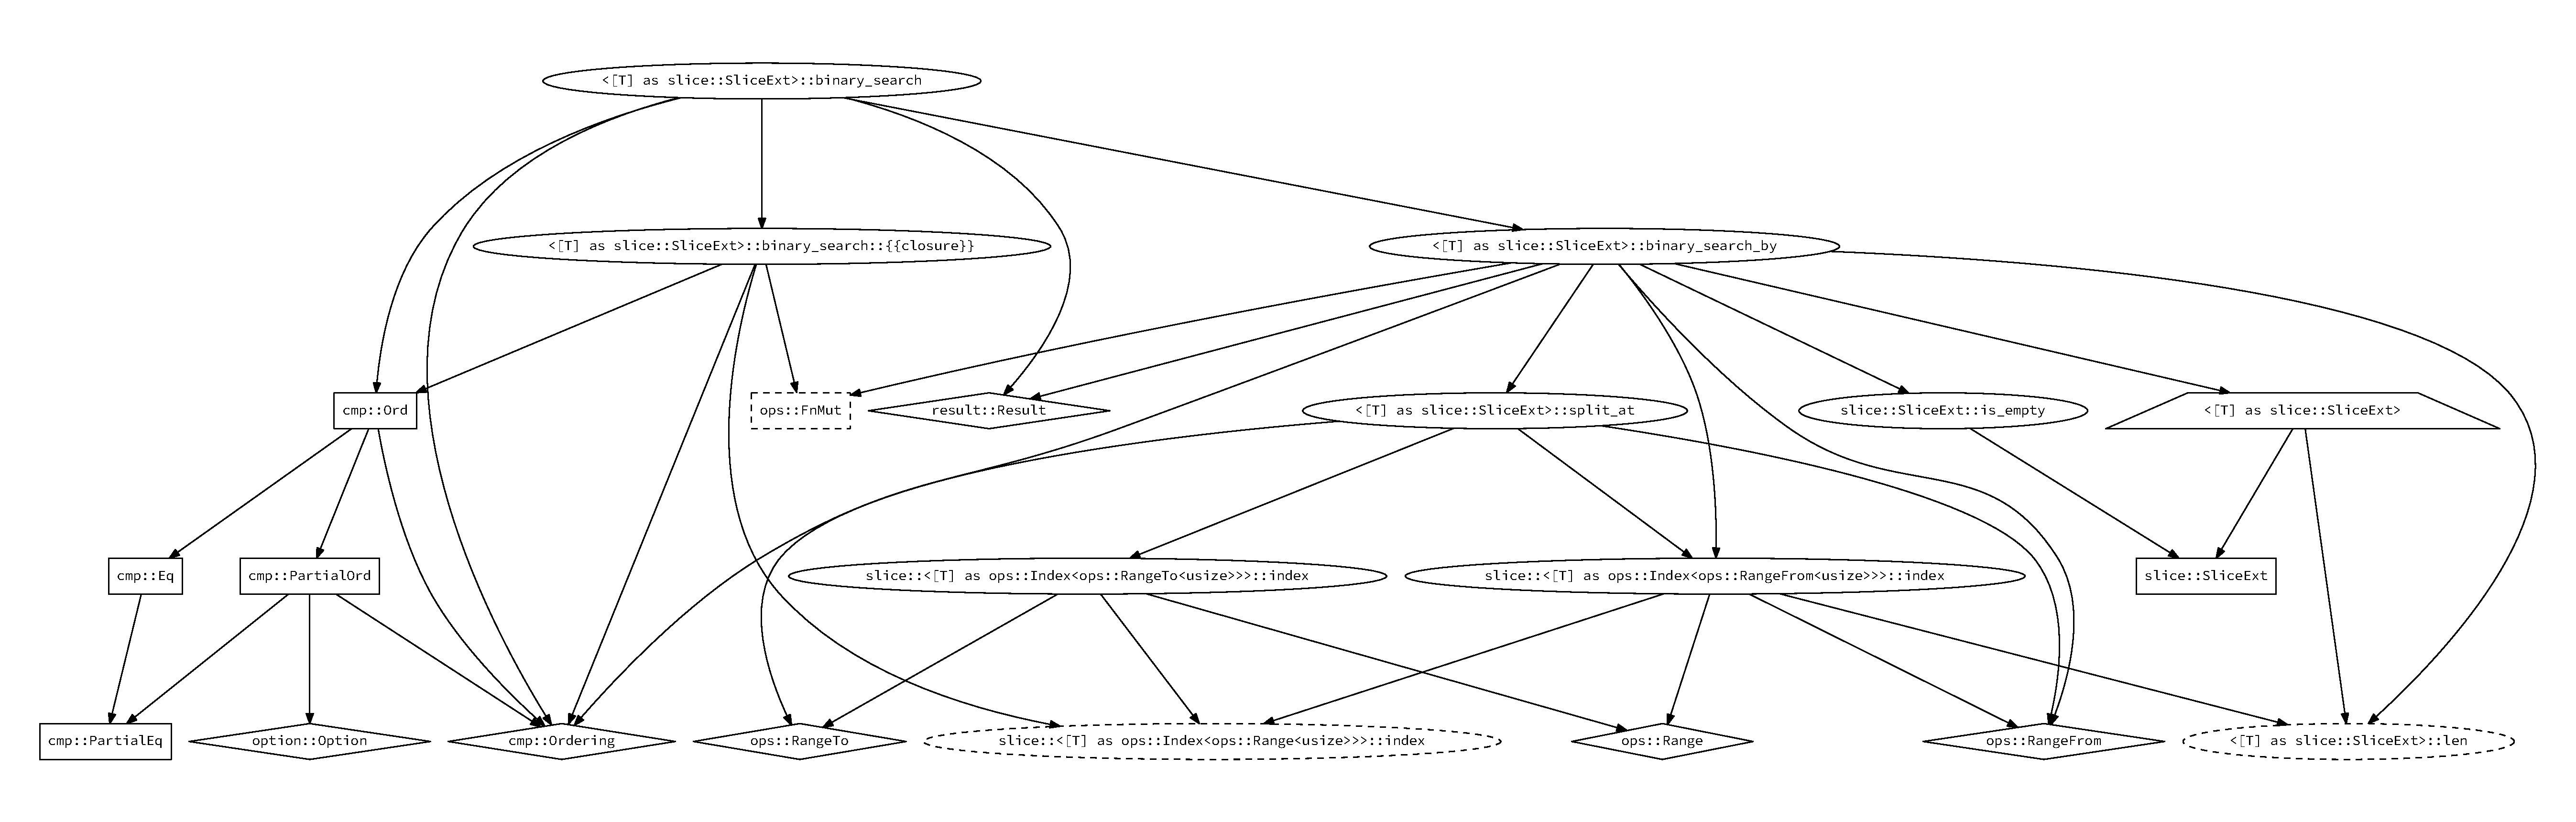
\includegraphics[width=\textheight]{deps}
  \caption[A complete graph of the dependencies of \rust{binary_search}]{A
    complete graph of the translation dependencies of \rust{binary_search} in
    the \rust{core} crate,
    distinguishing between \tikz[baseline=-0.3em]\node[draw, shape=ellipse] {functions};,
    \tikz[baseline=-0.3em]\node[draw, shape=rectangle] {types};,
    \tikz[baseline=-0.3em]\node[draw, shape=diamond, aspect=2] {traits};,
    and \tikz[baseline=-0.3em]\node[draw, shape=trapezium] {trait
      implementations};. Axiomatized definitions that use unsafe code in the original
    implementation are marked by dashed borders. Because
    we eagerly resolve trait method calls where possible, such as to the
    \rust{index} method of \rust{Index<RangeFrom<usize>>} for \rust{[T]}, we can
    avoid some dependencies like the full \rust{Index} implementation for
    \rust{[T]}, and even the trait itself.
  }
  \label{fig:deps}
\end{sidewaysfigure}
\restoregeometry

For our purposes, the abstract implementation primarily means a fair number of
additional dependencies we have to support and inspect~(\autoref{fig:deps}). All
in all, \rust{binary_search} turned out to be an ideal first test not only because
of its algorithmic complexity, but also because of its use of numerous Rust
language features including enums, structs, traits with associated types and
default methods, higher-order functions, and loops.

\subsection{Prelude: Coping with Unsafe Dependencies}

When trying to translate the \rust{binary_search} method including its
dependencies, we will not get back a definition at first. Our tool
refuses to translate some dependencies because they use unsafe code, as marked
in \autoref{fig:deps}. We will have to translate these functions manually,
basically adding the correctness of their translation as axioms to the project.

Apart from our custom translation of \rust{FnMut} we discussed in
\autoref{sec:lambda}, both axiomatized functions operate on slices and are straightforward to
implement using our identification of slices with Lean lists.

\begin{minted}{lean}
-- Returns the number of elements in the slice.
definition «[T] as core.slice.SliceExt».len {T : Type₁} (self : slice T) : sem nat :=
return (list.length self)

-- Implements slicing with syntax `&self[begin .. end]`.
-- Returns a slice of self for the index range [`begin`..`end`).
-- This operation is `O(1)`.
-- Requires that `begin <= end` and `end <= self.len()`,
-- otherwise slicing will panic.
definition «[T] as core.ops.Index<core.ops.Range<usize>>».index {T : Type₁} (self : slice T) (index : Range usize) : sem (slice T) :=
sem.guard (Range.start index ≤ Range.«end» index ∧ Range.«end» index ≤ list.length self)
  (return (list.firstn (Range.«end» index - Range.start index) (list.dropn (Range.start index) self)))
\end{minted}

The latter method presents a
small technical hurdle: It is dependent on other translation products,
specifically the \lean{Range} structure. Instead of having to axiomatize that
perfectly translatable definition too and adding both definitions manually to the
\verb!pre.lean! file, we instruct the translator in the \verb!config.toml! file to inject our
Lean definition of \rust{index} as the translation of the Rust definition on-the-fly.

\begin{minted}{text}
[replace]
"«[T] as core.ops.Index<core.ops.Range<usize>>».index" = "..."
\end{minted}

\subsection{Formal Specification}

Going back to the original definition of \rust{[T]::binary_search}, we translate
the documented behavior into a Lean predicate.

\begin{minted}{lean}
parameter {T : Type₁}
hypothesis [Ord T] -- a synonym for `parameter`
parameter self : slice T
parameter needle : T -- a more descriptive name for the parameter `x`

inductive binary_search_res : Result usize usize → Prop :=
| found     : Πi, list.nth self i = some needle → binary_search_res (Result.Ok i)
| not_found : Πi, needle ∉ self → sorted (list.insert_at self i needle) →
  binary_search_res (Result.Err i)
\end{minted}

It is specifications like these where the power of shallow embeddings really
shines: We can freely mix and match Rust types and standard Lean functions and
constructs. In fact, we will have to do some more mixing of these two worlds to make
the definition valid: While we have copied the assumption \rust{T : Ord} from
the \rust{binary_search} method, the \lean{sorted} predicate expects T to
implement Lean's own ordering type class. We therefore introduce a new type class
\lean{Ord'} that brings both type classes together -- or rather, in the Lean case, the
subclass of decidable, linear orders.

\begin{minted}{lean}
definition ordering {T : Type₁} [decidable_linear_order T] (x y : T) : cmp.Ordering :=
if x < y then Ordering.Less
else if x = y then Ordering.Equal
else Ordering.Greater

structure Ord' [class] (T : Type₁) extends Ord T, decidable_linear_order T :=
(cmp_eq : ∀ x y : T, Σ k, Ord.cmp x y = some (ordering x y, k))
\end{minted}

After changing the \lean{hypothesis} to \lean{[Ord' T]}, the
specification typechecks. We need two more (sensible) hypotheses before we can
prove that \lean{binary_search} upholds the specification.

\begin{minted}{lean}
hypothesis Hsorted : sorted self
hypothesis His_slice : is_slice self

...

theorem binary_search.spec : sem.terminates_with
  binary_search_res
  (binary_search self needle) := ...
\end{minted}

\subsection{Proof}

The full correctness proof is about 170 lines in Lean's tactic mode. We will not
discuss the individual steps or the Lean tactic syntax here, but focus on the main
proof steps.

After unfolding the \lean{binary_search} and \lean{binary_search_by}
definitions and some simplifications, we quickly reduce the proof obligation
down to the central loop.

\begin{minted}{lean}
⊢ sem.terminates_with binary_search_res
    (loop loop_4 (closure_5594.mk needle, 0, self))
\end{minted}

Here \lean{loop_4} is the loop body extracted from \lean{binary_search_by},
which is passed to the loop combinator \lean{loop} together with the initial
loop state. The loop state is the triple \lean{(f, base, s)} of local variables
mutated in the loop, initialized to the closure from \lean{binary_search}
(capturing \lean{needle}), \lean{0}, and \lean{self}, respectively. As described
in \autoref{sec:loop}, we can reduce the goal to one basing the loop on a
specific relation by use of the lemma \lean{loop.fix_eq_loop}.

\begin{minted}{lean}
abbreviation f₀ := closure_5594.mk needle
abbreviation loop_4.state := closure_5594 T × usize × slice T
definition R := measure (λ st : loop_4.state, length st.2)
...

⊢ sem.terminates_with binary_search_res
  (loop.fix loop_4 R (f₀, 0, self))
\end{minted}

The \lean{measure} function lets us create a well-founded relation on the loop state triple
by comparing the length of \lean{s}. We will not be able to show the new goal
directly via well-founded induction over \lean{R}, instead we first have to
generalize it. For that we first declare the loop invariants (which we obtained by
the non-sophisticated method of repeated try-and-error).

\begin{minted}{lean}
variables (base : usize) (s : slice T)

structure loop_4_invar :=
(s_in_self  : s ⊑ₚ dropn base self)
(insert_pos : sorted.insert_pos self needle ∈ '[base, base + length s])
(needle_mem : needle ∈ self → needle ∈ s)
\end{minted}

These say that
\begin{enumerate}
\item \lean{s} is a contiguous subsequence of the original slice \lean{self} starting at \lean{base}; here \lean{⊑ₚ} is a
  notation for the (non-strict) list prefix order that will come in handy at multiple points
  in the proof.
\item inserting \lean{needle} at the first position in \lean{self} that will
  keep it sorted will insert it inside or adjacent to \lean{s}.
\item if \lean{needle} is at all in the original slice, it will also be in
  \lean{s}. If this is the case, this invariant will imply the previous one, but in
  general they are independent.
\end{enumerate}

Because the invariants trivially hold for the initial state, we can generalize
the goal.

\begin{minted}{lean}
⊢ loop_4_invar base s → sem.terminates_with binary_search_res
    (loop.fix loop_4 R (f₀, base, s))
\end{minted}

There is no need to generalize \rust{f₀} because we know it is a non-modifying closure
and thus the variable \rust{f} will always contain that value.

After applying well-founded recursion, we unroll one iteration of
\lean{loop.fix} via the lemma \lean{loop.fix_eq} from \autoref{sec:loop} and
apply the induction hypothesis on the loop remainder to reduce the goal to that
single iteration.

\begin{minted}{lean}
inductive loop_4_step : loop_4.state → Prop :=
mk : Π base' s', loop_4_invar base' s' → length s' ≤ length s / 2 → length s ≠ 0 →
  loop_4_step (f₀, base', s')

abbreviation loop_4_res := sum.rec (loop_4_step s) binary_search_res

⊢ loop_4_invar base s → sem.terminates_with
    loop_4_res
    (loop_4 (f₀, base, s))
\end{minted}

If the iteration breaks the loop (returns some \lean{sum.inr}), we need the
result to fulfill the top-level specification \lean{binary_search_res}.
Otherwise, if the loop produces
some new loop state \lean{(f₀, base', s')}, the loop invariants should be upheld
together with a loop \emph{variant} saying that the length of \lean{s} has at
least halved. Together with the information that \lean{length s ≠ 0}, this
implies \lean{length s' < length s} and ensures we can apply the induction
hypothesis. We will
need the former two stronger statements for proving the function's logarithmic
complexity in \autoref{sec:asymptotic}.

The remainder of the proof, while tedious, uses mostly basic reasoning. We split
the goal according to the \rust{if} and \rust{match} branches in the original
code and, depending on the return value in each case, show that
\lean{loop_4_invar} or \lean{binary_search_res} is upheld. We prove that neither
of the two additions in the code overflows by showing that they are bounded by
\lean{list.length self}, which by the assumption \lean{is_slice self} fits into
the \rust{usize} type.
\newpage
\section{Transformation of Mutable References}
\label{sec:mutref}

As the previous section showed, the basic transformation already allows us to reason about mutability in
form of local variables, including inside loops. The next step is to support
indirect mutability in form of mutable references. We will develop
a restricted but extendable transformation of mutable references in this section
and put it to use in the next section.

\subsection{Lenses as Functional References}

In order to correctly translate mutable references, we will take a more careful
look at their structure in the MIR (\autoref{sec:mir}). Mutable references are
created by the \rust{&mut x} syntax, which in MIR operates on \emph{lvalues}.

\begin{minted}{rust}
pub enum Rvalue<'tcx> {
  /// &x or &mut x
  Ref(&'tcx Region, BorrowKind, Lvalue<'tcx>),
  ...
}
\end{minted}

An lvalue in Rust is either a local or static (global) variable, or inductively some
projection of another lvalue.

\begin{minted}{rust}
pub enum Lvalue<'tcx> {
    Local(Local),
    Static(DefId),
    /// projection out of an lvalue (access a field, deref a pointer, etc)
    Projection(Box<LvalueProjection<'tcx>>),
}
\end{minted}

Because mutable static variables are not allowed in safe Rust, we may assume
that every lvalue is rooted in a local variable. We can describe a mutable
reference as \emph{focusing} on some part of a local variable, which in
functional programming can represented by
\emph{lenses}~\cite{foster2005combinators} (also known as \emph{functional
  references}). For our purposes, a very simple presentation of lenses that
allows us to get and set the focused part is sufficient. We also specialize it
to return our semantics monad.

\begin{minted}{lean}
structure lens (Outer Inner : Type₁) :=
(get : Outer → sem Inner)
(set : Outer → Inner → sem Outer)
\end{minted}

Our lens type describes how some type \lean{Inner} can be extracted from and
replaced inside another type \lean{Outer}. For the correct combinations of those
two types, we can give some general instances such as identity and composition.

\begin{minted}{lean}
definition lens.id {Inner : Type₁} : lens Inner Inner :=
⦃lens, get := return, set := λ o, return⦄

definition lens.comp {A B C : Type₁} (l₂ : lens B C) (l₁ : lens A B) :
  lens A C :=
⦃lens, get := λ o,
  do o' ← lens.get l₁ o;
  lens.get l₂ o',
 set := λ o i,
  do o' ← lens.get l₁ o;
  do o' ← lens.set l₂ o' i;
  lens.set l₁ o o'⦄

infixr ` ∘ₗ `:60 := lens.comp
\end{minted}

We can now translate the \rust{&mut x} operation: We generate a lens per
projection, then compose them together to obtain a value of type \lean{lens A B}
where \lean{B} is the type of \lean{x}, and \lean{A} the type of the root variable of
\lean{x}. For the projection of indexing into an array or slice we can give a generic
definition, but for other projections such as struct fields we will have to
generate them at translation time.

\begin{minted}{lean}
definition lens.index (Inner : Type₁) (index : ℕ) :
  lens (slice Inner) Inner :=
⦃lens,
  get := λ o, sem.lift_opt (list.nth self o),
  set := λ o i, sem.lift_opt (list.update o index i)⦄
\end{minted}

There is one projection we have to special case: dereferencing an lvalue as in
\rust{*x}. If \rust{x} is an immutable reference, this is just the identity lens
because \rust{&T} and \rust{T} are translated to the same type (\autoref{sec:refs}). If it is a
mutable reference, we compose with its lens to obtain a lens on the ultimate
root variable. This combination of referencing and dereferencing is also known as ``reborrowing''.

\begin{sbs1}
let x: &mut [T] = &mut a;
let y = &mut (*x)[1];
\end{sbs1}
\begin{sbs2}
let x := lens.id in
let y := lens.index _ 1 ∘ₗ x in
...
\end{sbs2}

There is a final technicality involved with creating mutable references. Because
in Rust a reference is represented merely by an address, index projections are
checked to be in bounds when creating the reference, whereas \lean{lens.index}
will return \lean{mzero} only when its getter or setter is used. Therefore, we
``probe'' lenses eagerly after creation by invoking their getter in order to
make sure we exhibit the same termination behavior as the original code.

\subsection{Pointer Bookkeeping}
\label{sec:book}

In order to actually invoke \lean{lens.get} or \lean{lens.set}, we also need to
pass it the ``outer'' object, \ie the root variable of the original borrow. This
is not a kind of information we can dynamically save alongside the lens in the
mutable reference, but we instead have to statically determine at translation
time. For now, we represent this information as a mapping from variable names to
variable names.

\begin{minted}{rust}
let x: &mut [i32] = &mut a; // {'x' ~> 'a'}
// moving &mut
let x2 = x;                 // {'x2' ~> 'a'}
// reborrowing &mut
let y = &mut (*x2)[1];      // {'x2' ~> 'a', 'y' ~> 'a'}
\end{minted}

While this simple mapping has proved sufficient so far, it does impose
the following limitations:

\begin{itemize}
\item Mutable references can only be stored directly in variables, not nested in
  some structure. This also means that we do not have to worry about how to
  represent mutable references in type declarations, yet.
\item Whereas a completely static mapping works for linear code, it cannot work
  for variables that are part of a loop state in general. We could lift this
  restriction for the most common special case where the loop changes the lens,
  but not the root variable of a reference.
\end{itemize}

\subsection{Passing Mutable References}
\label{sec:passable}

In \autoref{sec:rust}, we introduced references as a more ergonomic (and
efficient) way of passing ownership of a value to some function and getting back the
old or (in the case of mutable references) new value from the function. While we
do not have to worry about ownership in Lean, we can still use the reverse pattern
for passing mutable references in Lean. For each mutable reference argument, we
read the current value through the lens, pass it to the function, get back the new
value as part of the return value, and write it back through the lens. Inside
the called function, we immediately re-wrap the value in the identity lens. This
is only correct because of the absence of mutable aliasing.

\begin{sbs1}
fn f(x: &mut T) -> R {...}
...

let x: &mut T =
  &mut ...a...;
let y = f(x);
\end{sbs1}
\begin{sbs2}
definition f : (xₐ : T) : sem (R × T) :=
let x := lens.id in -- {'x' ~> 'xₐ'}
...

let x = ... in
do tmp ← lens.get x a;
do ret ← f tmp;
match ret with
| (y, tmp) :=
  do a ← lens.set x a tmp;
  ...
end
\end{sbs2}

There is a small caveat with this approach: It does not work if a parameter's type is
declared to be a type parameter, but then instantiated to a mutable reference.

\subsection{Returning Mutable References}

While passing mutable references to functions has a rather simple desugaring,
returning them is a very different beast altogether: The caller has no idea
where the reference is pointing to. For now, we restrict ourselves to the
special case of returning
mutable references that point into the first parameter, which in particular covers all
methods that return references pointing into their \rust{&mut self} parameter.
We statically check this property when translating the callee, and then use that
knowledge in the caller to compose the returned lens with the lens of the first argument. Note
that we still have to return the new pointee for the first argument, as by the
previous subsection.

\begin{sbs1}
fn f(x: &mut T) -> &mut R {...}
...

let x: &mut T =
  &mut ...a...;
let y = f(x);
\end{sbs1}
\begin{sbs2}
definition f (xₐ : T) : sem (lens T R × T) :=
...

let x = ... in
do tmp ← lens.get x a;
do ret ← f tmp;
match ret with
| (y, tmp) :=
  let y := y ∘ₗ x in
  do a ← lens.set x a tmp;
  ...
end
\end{sbs2}

% \subsection{Discussion}
% 
% The astute reader may notice that our lens representation of mutable references
% does not actually make use of their uniqueness property; while we do utilize the
% absence of aliasing for representing the more common immutable references
% (\autoref{sec:refs}), two lenses focused one the same object could in theory
% coexist because they do not hold any state on their own.
% 
% We could indeed make use of the aliasing property by saving the state in the
% lens itself and writing it back only at the lens' end of lifetime.
% 
% \begin{minted}{lean}
% structure lens (Outer Inner : Type₁) :=
% (value : Inner)
% (set : Outer → Inner → sem Outer)
% \end{minted}
% 
% While this arguably simpler representation would save us a monadic bind when
% reading from a mutable reference, there are one technical reason and two arguments
% of future extensibility that made us go with the former representation. 
\newpage
\section{Case Study: Partial Verification of \texttt{FixedBitSet}}
\label{sec:fixedbitset}

Whereas our first case study focused on algorithmic verification, for our second
study we chose the \rust{FixedBitSet} data structure from the \rust{fixedbitset}
crate.\footnote{https://docs.rs/fixedbitset/} It can be thought of as
a more efficient version of a boolean array that stores elements packed at the bit
level. While it is not a complex data structure, verifying it does require
reasoning about the following important parts:

\begin{itemize}
  \item The ubiquitous \rust{Vec} type from the Rust standard library, which
    \rust{FixedBitSet} uses internally, including mutable references into it
  \item Data structure invariants
  \item Bitwise operations
\end{itemize}

\subsection{The Rust Implementation}

\rust{FixedBitSet} uses an internal \rust{Vec} to store up to 32 bits per element.

\begin{minted}{rust}
type Block = u32;

pub struct FixedBitSet {
  data: Vec<Block>,
  /// length in bits
  length: usize,
}
\end{minted}

We will focus on three basic operations: creating (\rust{with_capacity}),
manipulating (\rust{insert}), and querying (\rust{contains}) a
\rust{FixedBitSet}. The Rust implementations are shown in \autoref{lst:fixedbitset}.

\begin{listing}[!bt]
\begin{minted}{rust}
const BITS: usize = 32;
fn div_rem(x: usize, d: usize) -> (usize, usize) {
  (x / d, x % d)
}

impl FixedBitSet {
  pub fn with_capacity(bits: usize) -> Self {
    let (mut blocks, rem) = div_rem(bits, BITS);
    blocks += (rem > 0) as usize;
    FixedBitSet {
      data: vec![0; blocks],
      length: bits,
    }
  }

  pub fn insert(&mut self, bit: usize) {
    assert!(bit < self.length);
    let (block, i) = div_rem(bit, BITS);
    unsafe {
      *self.data.get_unchecked_mut(block) |= 1 << i;
    }
  }

  pub fn contains(&self, bit: usize) -> bool {
    let (block, i) = div_rem(bit, BITS);
    match self.data.get(block) {
      None => false,
      Some(b) => (b & (1 << i)) != 0,
    }
  }
  ...
}
\end{minted}

  \caption{The Rust implementations of the three methods}
  \label{lst:fixedbitset}
\end{listing}

\subsection{Prelude: Axiomatizing \texttt{collections::vec::Vec}}

\rust{Vec} is the standard type for dynamically-sized arrays in Rust. It is
implemented on top of an unsafe abstraction called \rust{RawVec} that handles
allocating, resizing, and deallocating the array memory. \rust{Vec} provides a
safe interface on top of that type by additionally keeping track of ownership of individual items
via a \rust{len} field. Elements after the first \rust{len} items are not
logically part of the \rust{Vec} and must be viewed as unitialized storage.

\begin{minted}{rust}
pub struct Vec<T> {
    buf: RawVec<T>,
    len: usize,
}
\end{minted}

Because \lean{Vec} provides a safe interface, but is itself implemented using
(predominantly) unsafe code, we both can and have to axiomatize it. When axiomatizing data structures, we are free to choose any abstraction as long
as the operations on it preserve their semantics. Just as with arrays and
slices, Lean's basic \lean{list} type is a natural representation for
\rust{Vec}.

\begin{minted}{lean}
structure Vec (T : Type₁) :=
(buf : list T)
\end{minted}

We do lose information about the \rust{RawVec}'s length (also called the
\rust{Vec}'s \emph{capacity}) here, but this information is not exposed by the
\rust{Vec} operations \rust{FixedBitSet} depends on. \autoref{lst:vec} lists the Lean implementations of
the needed \rust{Vec} methods, none of which should be surprising.

\begin{listing}[bt!]
\begin{minted}{lean}
namespace «Vec<T>»
  parameter {T : Type₁}

  definition new : sem (Vec T) :=
  return (Vec.mk [])

  -- note: only a runtime upper bound
  definition push (self : Vec T) (value : T) : sem (unit × Vec T) :=
  sem.incr (list.length (Vec.buf self)) (return (unit.star, Vec.mk (Vec.buf self ++ [value])))

  -- note: `pop` never resizes the `Vec`, so it is always constant-time
  definition pop (self : Vec T) : sem (Vec T × Option T) :=
  match reverse (Vec.buf self) with
  | x :: xs := return (Vec.mk (reverse xs), Option.Some x)
  | []      := return (self, Option.None)
  end

  definition clear (self : Vec T) : sem (Vec T) :=
  sem.incr (list.length (Vec.buf self)) new

  definition len (self : Vec T) : sem usize :=
  return (list.length (Vec.buf self))
end «Vec<T>»
\end{minted}
  
  \caption{Axiomatizations of relevant \rust{Vec} methods}
  \label{lst:vec}
\end{listing}

\rust{Vec} also implements the \rust{Deref} trait, which makes values of type
\rust{&Vec<T>} automatically coerce to \rust{&[T]} and is implicitly being used
in \rust{FixedBitSet::contains}. This is easy enough to implement using our abstraction.

\begin{minted}{lean}
definition «collections.vec.Vec<T> as core.ops.Deref».deref {T : Type₁} (self : Vec T) :
  sem (slice T) :=
return (Vec.buf self)
\end{minted}

There is also a corresponding \rust{DerefMut} trait that makes \rust{&mut
  Vec<T>} coerce to \rust{&mut [T]}. The implementation is slightly more
interesting because it has to return a lens focusing on \lean{Vec.buf}.

\begin{minted}{lean}
definition «collections.vec.Vec<T> as core.ops.DerefMut».deref_mut {T : Type₁} (self : Vec T) :
  sem (lens (Vec T) (slice T) × Vec T) :=
return (⦃lens, get := return ∘ Vec.buf, set := λ old, return ∘ Vec.mk⦄,
        self)
\end{minted}

This trait implementation is being being used by \rust{FixedBitSet::insert} to
access \rust{[T]::get_unchecked_mut}, which in turn returns a mutable reference
to a single slice element.

\begin{minted}{lean}
definition «[T]».get_unchecked_mut {T : Type₁} (self : slice T) (index : usize) :
  sem (lens (slice T) T × slice T) :=
sem.guard (index < length self) (return (lens.index _ index, self))
\end{minted}

This method is interesting in that it actually is unsafe to call in Rust --
instead of an explicit panic, an out-of-bounds access will silently invoke
undefined behavior.

\begin{minted}{rust}
unsafe fn get_unchecked_mut(&mut self, index: usize) -> &mut T {
    &mut *self.as_mut_ptr().offset(index as isize)
}
\end{minted}

There is also a safe, panicking variant called \rust{[T]::get_mut}, which we
first mentioned in \autoref{sec:related} as not being expressible in other
verifiable languages. Because our semantics monad does not currently differentiate between
undefined behavior and panics, both functions become semantically equivalent in
our transformation and we can translate calls to both of them, including the
small bit of unsafe code in \rust{FixedBitSet::insert}.

\subsection{Formal Specification}

There is no useful abstract specification we could give \rust{contains} without
essentially restating its implementation. Instead, we use it to \emph{build} an
abstraction: We translate \rust{FixedBitSet} to a Lean set of indices.

\begin{minted}{lean}
abbreviation sem.returns {A : Type₁} (x : A) := sem.terminates_with (λ a, a = x)

open FixedBitSet

definition to_set (s : FixedBitSet) : set usize :=
{bit | bit < length s ∧ sem.returns bool.tt (contains s bit)}
\end{minted}

The additional constraint \lean{bit < length s} may seem superfluous considering
that \lean{contains} makes sure to always return \rust{false} for indices after
the last \rust{u32} block. However, indices between the length and the capacity
may not necessarily be \rust{false}, as noted in the docstring for a different method:

\begin{minted}{rust}
/// View the bitset as a mutable slice of `u32` blocks. Writing past the
/// bitlength in the last block will cause `contains` to return
/// potentially incorrect results for bits past the bitlength.
pub fn as_mut_slice(&mut self) -> &mut [u32]
\end{minted}

%To make the definition meaningful, we also show that \rust{contains} does
%indeed terminate (for any index).
With \lean{to_set}, we can give \rust{insert} a natural specification using
standard Lean \lean{set} operations.

\begin{minted}{lean}
lemma insert.spec (s : FixedBitSet) (bit : usize) : bit < length s →
  sem.terminates_with
    (λ ret, to_set ret.2 = to_set s ∪ '{bit})
    (insert s bit)
\end{minted}

To prove this lemma, we will also need a data type invariant on \rust{FixedBitSet} relating its two
fields: The \rust{Vec} should always have the minimum length, that is, the
number of bits divided by 32, then rounded up. As with traits, we specify the
invariant as a type class.

\begin{minted}{lean}
structure FixedBitSet' [class] (self : FixedBitSet) : Prop :=
(length_eq : nat.div_ceil (length self) 32 = list.length (Vec.buf (data self)))
\end{minted}

This invariant should be fulfilled by the constructor, \rust{with_capacity}.

\begin{minted}{lean}
lemma with_capacity_inv (bits : usize) [is_usize bits] :
  sem.terminates_with FixedBitSet' (with_capacity bits)
\end{minted}

After adding the hypothesis \lean{[FixedBitSet' s]} to \lean{insert.spec}, the
lemma becomes provable. We also show that the invariant is upheld, \ie that
\lean{FixedBitSet' s'} holds.

\subsection{Proof}

We will focus on the correctness proof of \lean{insert}. With 77 lines, it is
quite shorter (and simpler) than the binary search proof, so we will show some
more details, including some reasoning about bitwise operations.

We again start by unfolding definitions and simplifying the resulting goal. We
also eliminate some bounds checks, introducing \lean{bit_block} for the \rust{u32} block
\lean{bit} is part of, and \lean{l'} and \lean{s'} for the updated list and
\lean{FixedBitSet}, respectively.

\begin{minted}{lean}
...
bit_block : ℕ,
bit_block_eq : list.nth (Vec.buf (FixedBitSet.data s)) (bit / 32) = some bit_block,
l' : list ℕ,
l'_eq : list.update (Vec.buf (FixedBitSet.data s)) (bit / 32) (bit_block ||[32] 2 ^ (bit % 32)) = some l',
s' : FixedBitSet,
s'_eq : s' = FixedBitSet.mk (Vec.mk l') (FixedBitSet.length s)
⊢ FixedBitSet' s' ∧ to_set s' = to_set s ∪ '{bit}
\end{minted}

Here the notation \lean{||[32]} is an abbreviation for \lean{bitor 32}. We show the data type invariant by a helper lemma saying that
\lean{list.length} is invariant under \lean{list.update}. After unfolding
\lean{to_set} and some more simplifications, we are left with a
goal that asserts that some index \lean{bit'} is in the new set iff it is in
the old set or is equal to \lean{bit}.

\begin{minted}{lean}
...
bit' : ℕ
⊢ bit' < FixedBitSet.length s ∧ sem.returns bool.tt (FixedBitSet.contains s' bit') ↔
  bit' < FixedBitSet.length s ∧ sem.returns bool.tt (FixedBitSet.contains s bit') ∨ bit' = bit
\end{minted}

If \lean{bit'} is not a valid index (\lean{bit' ≥ FixedBitSet.length s}), the
goal reduces to \lean{bit' ≠ bit}, which holds because \lean{bit} is assumed to
be valid. If, on the other hand, \lean{bit'} is valid, we will have to reason
about the two \lean{contains} calls. After unfolding them and some more
simplifications, we are left with a bit-level goal talking about the
\rust{u32} block for \lean{bit'} in the old set (\lean{bit'_block}) and in the
new set (\lean{bit'_block'}), respectively.

\begin{minted}{lean}
...
bit'_block bit'_block' : ℕ,
bit'_block_eq : list.nth (Vec.buf (FixedBitSet.data s)) (bit' / 32) = some bit'_block,
bit'_block'_eq : (if bit / 32 = bit' / 32 then some (bit_block ||[32] 2 ^ (bit % 32)) else some bit'_block) = some bit'_block'
⊢ bit'_block' &&[32] 2 ^ (bit' % 32) ≠ 0 ↔
  bit'_block &&[32] 2 ^ (bit' % 32) ≠ 0 ∨ bit' = bit
\end{minted}

We proceed by splitting the goal according to the conditional in
\lean{bit'_block'_eq}. In the case \lean{bit / 32 ≠ bit' / 32}, we obtain
\lean{bit'_block' = bit'_block} and \lean{bit' ≠ bit}, closing the goal. In less
formal words, \lean{bit'} turned out to be in a block entirely unaffected by the
whole insertion.

In the other case, we get \lean{bit'_block = bit_block} and the goal reduces to
a proposition about two bits in the same block.

\begin{minted}{lean}
⊢ (bit_block ||[32] 2 ^ (bit % 32)) &&[32] 2 ^ (bit' % 32) ≠ 0 ↔
  bit_block &&[32] 2 ^ (bit' % 32) ≠ 0 ∨ bit' = bit
\end{minted}

Assuming \lean{bit' = bit}, we see that both sides of the equivalence become universally true.
Otherwise, if \lean{bit' ≠ bit}, but \lean{bit / 32 = bit' / 32} by the previous
assumption, we obtain \lean{bit' % 32 ≠ bit % 32}. A helper lemma proves that this cancels
out the bitwise or and thus reduces both sides to the same term, concluding the proof.
\newpage
\section{Conclusion and Future Work}

\newpage
\bibliographystyle{abbrv}
\bibliography{bib}

\cleardoublepage
\pagestyle{empty}
\section*{Erklärung}

  \vspace{20mm}
  Hiermit erkläre ich, Sebastian Andreas Ullrich, dass ich die vorliegende Masterarbeit selbst\-ständig
verfasst habe und keine anderen als die angegebenen Quellen und Hilfsmittel
benutzt habe, die wörtlich oder inhaltlich übernommenen Stellen als solche kenntlich gemacht und
die Satzung des KIT zur Sicherung guter wissenschaftlicher Praxis beachtet habe.
  \vspace{20mm}
  \begin{tabbing}
  \rule{4cm}{.4pt}\hspace{1cm} \= \rule{7cm}{.4pt} \\
 Ort, Datum \> Unterschrift
  \end{tabbing}

\end{document}
